%%% -*-LaTeX-*-
\documentclass[../../Dissertation]{subfiles}

% Import a PDF and add sections to the table of contents, list of figures, and
% list of tables

\begin{document}

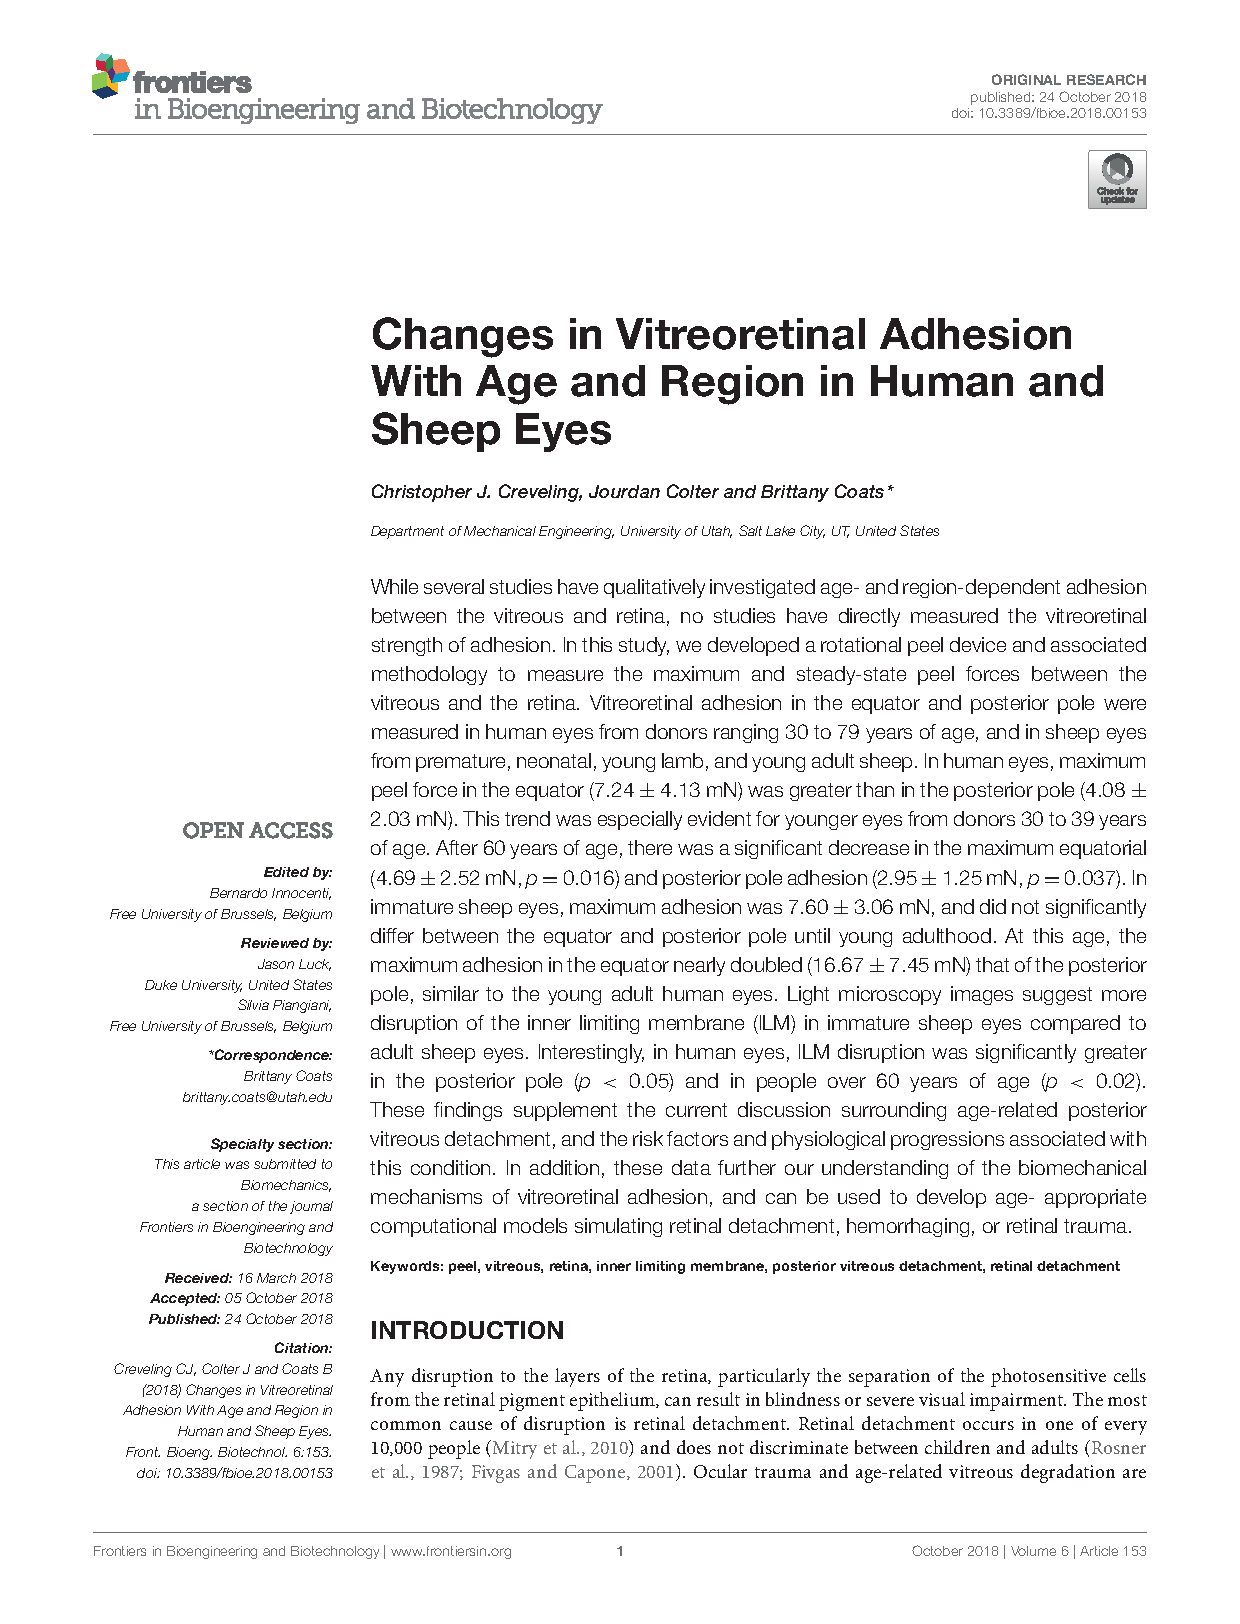
\includepdf[pagecommand={},
pages={1-},
addtotoc={
    1,section,1,Abstract,chp3A,   
    1,section,1,Introduction,chp3I,   
    2,section,1,Methods,chp3M,   
    2,subsection,2,Materials,chp3M_1,   
    3,subsection,2,Peel Test Setup and Protocol,chp3M_2,   
    4,subsection,2,Peel Test Validation,chp3M_3,   
    4,subsection,2,Data Analysis,chp3M_4,   
    5,section,1,Results,chp3R,   
    5,subsection,2,Effect of Age and Region in Sheep Eyes,chp3R_1,   
    6,subsection,2,Effect of Age and Region in Human Eyes,chp3R_2,   
    6,subsection,2,Locations of Failure,chp3R_3,   
    7,section,1,Discussion,chp3D,   
    10,section,1,Conclusion,chp3C,   
    10,section,1,References,chp3Ref},   
addtolist={
    3,figure,{(A) Scleral dissection methods used to create a rectangular
        retinal window (gray crosshatch) in the (B) equatorial and (C)
        posterior regions. The location of the optic nerve head is shown as a
        white circle, and the fovea marked with an ``x''.},3fig1,   
    4,figure,{For each peel test, (A) sclera was dissected away from the
        retina prior to testing, and the eye placed in the fixture. The eye was
        raised toward the testing window by inflating a polymer liner with air.
        (B) An L-shaped tab was glued to the retina and raised to peel the
        retina from the vitreous while measuring force. (C) Optical coherence
        tomography image of the peeled retina indicating separation was at the
        vitreoretinal interface and glue penetration was minimal.},3fig2,   
    4,figure,{(A) Tape linear peel tests were performed and compared to (B)
        tape rotational peel tests to ensure validity of the custom rotational
        peel device.},3fig3,   
    5,figure,{Average peel force measurements from the rotational tests were
        within 1.3\% of the average peel forces measured from linear peel tests
        using ASTM standard D6862-11. Only one rotational peel test is plotted
        for clarity.},3fig4,   
    6,figure,{Representative peel test showing peel force over time for a
        sheep specimen. Steady-state (SS) peel region started after maximum
        peel force was reached and ended before the retina began to fail.
        Steady-state peel force was calculated by averaging forces during the
        steady-state peel period. (B) Still image taken from the webcam video
        of a sheep retina peeling away from the vitreous at 90$^\circ$ during
        the steady-state peel region.},3fig5,   
    6,figure,{(A) Maximum and (B) steady-state peel forces for each sheep age
        group and region. Error bars indicate standard deviation from the mean
        ($*p = 0.0016$ and $^{**}p < 0.0001$).},3fig6,   
    7,figure,{(A) Maximum peel force for human specimens by age group and
        region. Error bars indicate standard deviation from the mean ($^*p <
        0.03$).  (B) Equatorial maximum peel force was significantly reduced
        after 60 years of age ($p < 0.01$). Bars indicate mean data prior to
        and including 60 years of age, and after 60 years of age.},3fig7,   
    7,figure,{Steady-state peel force in the equator of the youngest human
        eyes was significantly greater than the posterior pole, and
        significantly greater than the equatorial steady-state adhesion of all
        other ages. Error bars indicate standard deviation from the mean. $^*p
        < 0.002$ and $^{**}p < 0.015$.},3fig8,   
    8,figure,{(A–C) Light microscopy images of peeled sheep retinas indicate
        (A) failure primarily occurred at the ILM. (B) In some images, focal
        ILM disruption was noted, (C) particularly in the presence of blood
        vessels. There were no regional differences in failure location, but
        immature sheep eyes tended to have more ILM disruption than young adult
        sheep eyes. (D–F) For human eyes, (D) peeling in the posterior pole
        typically disrupted the ILM, (E) while peeling in the equator had a
        clean separation between the vitreous and retina.  (F) This clean
        separation was sometimes accompanied by traction-like undulations on
        the retinal surface.},3fig9},
scale=0.8]
{./Chapter3/media/fbioe-06-00153}

\end{document}

